\documentclass[11pt]{article}

\usepackage[utf8]{inputenc}
\usepackage[T1]{fontenc}
\usepackage{mathptmx}
\usepackage{microtype}
\usepackage[margin=1in]{geometry}
\usepackage{amsmath,amssymb,amsthm}
\usepackage{booktabs}
\usepackage{graphicx}
\usepackage{xcolor}
\usepackage{listings}
\usepackage[numbers,sort&compress]{natbib}
\usepackage[colorlinks=true,linkcolor=blue!50!black,citecolor=blue!50!black,urlcolor=blue!50!black]{hyperref}

\newtheorem{lemma}{Lemma}
\newtheorem{proposition}{Proposition}
\theoremstyle{remark}
\newtheorem{remark}{Remark}

\newcommand{\act}{E}
\newcommand{\dist}{D_g}
\newcommand{\R}{\mathbb{R}}

\lstset{
  basicstyle=\ttfamily\small,
  breaklines=true,
  frame=single,
  columns=fullflexible,
  keepspaces=true,
  showstringspaces=false
}

\title{The Relativistic Cognitive Field:\\
A Gravity-Inspired Activation Model for Memory Retrieval\\
with Validated Mass, Contradiction Valence and Decay}

\author{Goce Balgurov\\
\texttt{balgurov@giji.agency}}

\date{October 2026}

\begin{document}
\maketitle

\begin{abstract}
The central hypothesis of this paper is the author's physical claim: intelligence is an active force in the universe; information is a substance with an equivalence to energy; cognitive structures exert gravity and perform work in an $N$-dimensional space, and this organisation affects outcomes in the material world. We state it explicitly as a proposed physical framework and hypothesis, not as a proven result. To make it computable we introduce the \emph{Relativistic Cognitive Field} (RCF) and demonstrate its static memory-scoring formulation. Where a plain similarity-only vector retriever treats each stored item as an unweighted, stance-blind, timeless point ranked by distance alone, the RCF gives each stored pattern a \emph{rest mass} that starts at a small floor and grows only through human validation, a query-dependent \emph{valence} that is negative for patterns contradicting the query's intent, a query-warped diagonal metric, and a decay whose rate falls with mass and is reset by reinforcement. We prove the elementary properties of the computational model: activation is bounded in exact arithmetic; its logarithm decomposes into four retrieval signals (prior, interaction, distance, mass-scaled recency); with equal positive mass, $g\equiv 1$, equal valence, equal $\Delta t$ and unit-norm vectors it ranks exactly as cosine similarity; and the smoothing constant $\epsilon$ is the exchange rate between mass and proximity. Contradictions are retrieved by activation \emph{magnitude} and handed to a rule core with a three-valued label rather than suppressed or averaged away. A portable reference implementation reproduces every number, table and figure of the static worked example. The continuous dynamic field and the extension to physical systems are formulated as design and as testable hypotheses, not as results.
\end{abstract}

\section{Introduction}

In the author's reading of modern physics and computational science, thought is treated as an invisible byproduct, an epiphenomenon that leaves no mathematical trace: intelligence is not part of the fundamental equations that describe the universe, and the material world is modelled as if consciousness played no active, structural role in shaping it. This is the author's motivating perspective, not a survey of those disciplines.

This central hypothesis challenges that omission: \emph{intelligence is an active force in the universe; information is a substance with an equivalence to energy; cognitive structures exert gravity and perform work in an $N$-dimensional space, and this organisation affects outcomes in the material world.} This is the author's physical claim and the overarching hypothesis of the paper; it is proposed here as a physical and architectural framework to be tested, not presented as an established physical law.

To make this framework concrete and falsifiable, we separate what is proposed as physical theory from what is demonstrated computationally in this release. Section~\ref{sec:physical_claim} states the physical claim, maps the primitives of the cognitive field onto physical counterparts, proposes tests of its computational consequences, and states what a discriminating physical test would require. Sections~\ref{sec:model}--\ref{sec:execution} present the demonstrated part of the work: a static, computable memory-scoring model for an autonomous agent, with formal mathematical properties and a portable Python/NumPy reference implementation. Appendix~\ref{sec:dynamic_field} formulates the continuous $N$-body dynamic cognitive field as a theoretical design for future implementation.

A plain similarity-only retriever, the baseline of many retrieval-augmented systems and vector databases, represents knowledge as coordinates in an embedding space and ranks by a similarity metric alone, usually cosine or Euclidean distance \citep{reimers2019sbert,karpukhin2020dpr}; hybrid systems add priors, recency or learned ranking features (Section~\ref{sec:related}). Three properties of that plain baseline are limiting for an autonomous agent that must reason over its own memory. First, the space is \emph{massless}: a verified operating rule and an unverified web fragment have the same baseline weight, and only their distance to the query decides which is retrieved. Second, similarity is \emph{stance-blind}: a statement and its negation share almost all their tokens and therefore most of their embedding, and neural retrievers largely fail to tell them apart \citep{weller2024nevir}. Third, the space is \emph{timeless}: nothing fades, so stale and current entries compete on equal terms.

We propose to treat retrieval as the evaluation of a field rather than as sorting by distance. Each stored pattern is a body with a rest mass that starts at a fixed floor and grows only through human validation; a query warps the metric of the space along the axes that matter to it; opposing patterns carry a negative valence; and the activation of every body decays unless it is reinforced. We call the resulting model the \emph{Relativistic Cognitive Field} (RCF).\footnote{In psychology, ``field'' and ``valence'' originate with Kurt Lewin's topological field theory \citep{lewin1936principles}. The RCF is also distinct in content from recent 2026 preprints on ``Cognitive Field Theory'' (arXiv:2601.10221) and ``Cognitive Field Networks'' (arXiv:2609.16752).} In the demonstrated static computational model, the gravitational name describes the functional form of the potential: it borrows the inverse-square distance law and a mass-dependent potential from gravitation, without using Lorentz invariance, spacetime curvature, or field equations, and without pattern--pattern interaction. Section~\ref{sec:limits} states what physical gravity has that the static computational model does not yet implement.

The computational hypothesis of this paper is that a single activation function combining validated mass, signed valence, a query-warped metric and reinforcement-reset decay is a better substrate for agent memory than massless similarity, and that it degrades gracefully to standard practice when its extra terms are switched off. We do not test empirical benchmark superiority here. The contributions of this paper are:
\begin{enumerate}
  \item a formal statement of the physical claim and its mapping to the field primitives, together with proposed tests of its consequences and the requirements for a discriminating physical test (Section~\ref{sec:physical_claim});
  \item a precise statement of the static activation function with the assumptions under which it is well defined (Section~\ref{sec:model});
  \item its elementary mathematical properties with proofs: exact-arithmetic boundedness, a log-linear decomposition into four classical retrieval signals, reduction to a ranking equivalent to cosine similarity, and the role of the smoothing constant as a mass--proximity exchange rate (Section~\ref{sec:properties});
  \item sign semantics for contradiction: retrieval by activation magnitude with a three-valued label passed to a rule core (Section~\ref{sec:valence}), and a mass-dependent decay reset by reinforcement (Section~\ref{sec:decay});
  \item a worked example with a portable reference implementation that reproduces every number, table and figure of the worked example (Section~\ref{sec:example}), a statement of computational limitations and falsification experiments (Section~\ref{sec:limits}), and a design appendix formulating the continuous dynamic field (Appendix~\ref{sec:dynamic_field}).
\end{enumerate}

\section{The Physical Claim}
\label{sec:physical_claim}

\subsection{Statement of the Claim}
The physical hypothesis proposed by the author is that \emph{intelligence is an active force in the universe; information is a substance with an equivalence to energy; cognitive structures exert gravity and perform work in an $N$-dimensional space, and this organisation affects outcomes in the material world.} Under this hypothesis, when an intelligent system or human mind validates, organises, and reinforces information, it is not merely rearranging passive symbols; it is concentrating an information-theoretic substance that shapes the trajectory of subsequent states and decisions, and through action and physical coupling, alters material outcomes. This section states how the mathematical primitives of the RCF map onto this hypothesis and which tests are proposed. No physical experiments are reported in this paper, and the proposed tests do not yet discriminate the physical claim from an ordinary computational reading of the equations (Section~\ref{sec:physical_tests}).

\subsection{Mapping the Cognitive Field to the Physical Hypothesis}
The RCF formalises four primitives that serve simultaneously as computable scoring variables (Section~\ref{sec:model}) and as operational analogues of the physical claim:
\begin{itemize}
  \item \textbf{Rest mass ($m_i$) and information--energy equivalence:} In the static field, every pattern starts at the ingestion floor $m_0 > 0$, and mass above that floor is added only through human validation. Under the physical hypothesis, validated information carries an effective rest mass proportional to the irreversible cognitive and thermodynamic work invested in verifying and anchoring it, resisting perturbation and anchoring surrounding states.
  \item \textbf{Metric tensor ($g(Q)$) and dimensional work:} An active intent or query $Q$ supplies a non-negative diagonal metric tensor $g(Q)$ that stretches task-relevant dimensions and compresses irrelevant ones in the $N$-dimensional state space ($\dist(q,p_i) = \sum_{j=1}^d g_j(Q)(q_j - p_{ij})^2$). In the dynamic extension (Appendix~\ref{sec:dynamic_field}), sustained attraction performs structural work by permanently shifting the rest coordinates $r_i$ of stored patterns (hysteresis).
  \item \textbf{Potential energy ($\act(P_i,Q)$) and signed valence ($\gamma_i(Q)$):} The activation $\act(P_i,Q)$ represents the effective potential exerted by pattern $P_i$ at query position $q$. Unlike passive scalar potentials, cognitive interaction carries stance: alignment ($\sigma_i = +1$) attracts a state toward synthesis, while contradiction ($\sigma_i = -1$) exerts an opposing sign that must be resolved by explicit work rather than cancelled by linear averaging.
  \item \textbf{Entropic decay ($\lambda_i$) and inertial retention:} Unreinforced patterns lose effective activation exponentially at rate $\lambda_i = \lambda_0 / (1 + m_i/m_\ast)$. High-mass structures exhibit greater effective inertia against entropic relaxation, coupling informational permanence directly to accumulated validation mass.
\end{itemize}

\subsection{Proposed Tests of Computational Consequences and Candidate Physical Realisations}
\label{sec:physical_tests}
The tests below probe consequences of organising a system by the field, and candidate physical realisations of it. They are proposed, not run. A positive outcome would show that the organisation has the stated consequence; by itself it would not establish informational substance, energy equivalence or cognitive gravity, because lower energy per decision, better control and persistent substrate change can all follow from ordinary computational organisation. A negative outcome would reject the particular encoding, controller, implementation or task, not the hypothesis as a whole. A discriminating physical test still requires an operational mapping with units between validation mass and physical work, a specified conventional null model, a measurable quantitative prediction and a rejection criterion; this paper does not yet supply them.
\begin{enumerate}
  \item \textbf{Thermodynamic and Landauer-scale coupling:} If validated information possesses a systematic equivalence to physical energy beyond standard bit-erasure bounds, then physical memory substrates or biological/artificial reasoning systems operating under RCF-structured consolidation (high-mass anchoring and hysteresis) must exhibit a measurable difference in dissipated work or state-transition efficiency per resolved decision compared with unstructured (massless) storage at equal bit capacity. If all energetic effects reduce identically to hardware-level bit operations independent of cognitive organisation, this test gives the energy-equivalence claim no support beyond a control-theoretic reading.
  \item \textbf{Macroscopic material outcomes under controlled intervention:} The claim asserts that cognitive field organisation affects outcomes in the material world. In a closed-loop physical control or human--machine decision environment where actions have measurable physical work or error outcomes, agents governed by mass-validated, contradiction-aware field organisation ($m_i$, $g(Q)$, $|\act|$) must produce statistically significant reductions in physical action error or wasted physical work compared with massless similarity baselines under identical sensor/actuator physics. Failure to alter downstream physical outcomes would reject that implementation's claim to perform effective material work.
  \item \textbf{Hysteresis and structural persistence in physical substrates:} In the dynamic design (Appendix~\ref{sec:dynamic_field}), teaching inputs perform irreversible structural work on rest positions ($r_i \leftarrow r_i + \eta\delta_i$). When mapped onto physical associative substrates (such as neuromorphic or physical relaxation networks), repeated structured inputs must leave a measurable, mass-dependent hysteresis in the substrate's relaxation landscape that improves subsequent trajectory convergence; if the substrate relaxes without memory of validation mass, that realisation fails to exhibit cognitive gravity.
\end{enumerate}

\section{Related Work}
\label{sec:related}

\paragraph{Gravity and inverse-distance kernels in retrieval.}
The inverse-square form is one of the earliest spatial interpolation kernels in computing \citep{shepard1968two}. \citet{shi2005gravitation} proposed a gravitation-based retrieval model that treats documents and query terms as bodies with masses and derives a ranking function from their mutual attraction; related data-gravitation models weight distance by data mass and attribute weights in classification \citep{peng2005gravitation,peng2009dgc,cano2013dgc}, and \citet{salha2019gravity} use a log-mass minus log-squared-distance gravity decoder for graphs. The RCF shares the inverse-square distance but differs in what carries mass (human validation above a fixed floor, not term or degree statistics), in the signed valence, and in the decay term.

\paragraph{Document priors and authority.}
Giving entries a query-independent weight is standard: prior probabilities in language-model retrieval \citep{kraaij2002importance}, link-based authority \citep{page1999pagerank}, and the static features of learning-to-rank systems \citep{liu2009ltr}. The rest mass $m_i$ is such a prior, restricted by design to a fixed ingestion floor plus evidence of human validation.

\paragraph{Recency and forgetting.}
Time-aware ranking appears in time-based language models \citep{li2003time}. In cognitive architectures the base-level activation of a memory chunk decays as a power law of time since its uses \citep{anderson1991reflections,anderson2004integrated}, following the classical forgetting curve \citep{ebbinghaus1885}. Three recent agent-memory systems are the closest prior work to the RCF: the retrieval score of generative agents is a weighted sum of recency (exponential decay since last access), an LLM-rated importance, and cosine relevance \citep{park2023generative}; MemoryBank updates memory strength with an Ebbinghaus-style curve that depends on elapsed time and on each memory's importance \citep{zhong2024memorybank}, and \citet{hou2024agent} pair cosine relevance with an exponential retention whose time constant grows with each recall. The RCF combines the same three signals multiplicatively rather than additively (yielding the same log-linear structure as ACT-R's additive base-level, spreading, and mismatch terms \citep{anderson2004integrated}), derives its importance term from human validation above a fixed floor rather than a model's rating, makes the decay rate itself a function of mass, and adds a signed interaction term that those systems lack.

\paragraph{Query-dependent metrics.}
A diagonal metric $\sum_j g_j (q_j-p_{ij})^2$ is a Mahalanobis distance with a diagonal matrix. Learning such metrics from side information is well studied \citep{xing2003distance,goldberger2005nca,weinberger2009lmnn}, and context-dependent dimension salience is foundational in cognitive models of conceptual spaces and attention-weighted similarity \citep{nosofsky1986attention,shepard1987universal,gardenfors2000conceptual}; making the weights depend on the query is the per-dimension analogue of the query-conditioned weighting performed by attention \citep{vaswani2017attention}. We claim no novelty for the form of $g(Q)$; its role in the RCF is to counteract distance concentration (Section~\ref{sec:properties}).

\paragraph{Contradiction and negation.}
Detecting contradiction between texts is a recognised task \citep{demarneffe2008finding}, usually cast as natural-language inference \citep{williams2018mnli}. Counter-argument retrieval seeks the best opposing argument to a given one \citep{wachsmuth2018retrieval}. NevIR shows that most neural retrievers rank a passage and its negation almost at random \citep{weller2024nevir}. The RCF's valence term presupposes an external contradiction detector; what the field adds is the retrieval policy (magnitude, not sign) and the hand-off of the sign to a rule core.

\paragraph{Associative memory.}
Dense associative memories retrieve stored patterns through an energy function over the pattern set \citep{krotov2016dense,ramsauer2021hopfield}, MINERVA~2 sums probe--trace similarity into an echo intensity \citep{hintzman1984minerva,hintzman1986schema}, and spreading-activation theories \citep{collins1975spreading}, surveyed for IR by \citet{crestani1997spreading}, describe retrieval as activation propagating through a network. These are interactive models, which the static RCF is not; Section~\ref{sec:limits} and Appendix~\ref{sec:dynamic_field} discuss the relation.

\section{The Static Computational Field}
\label{sec:model}

\subsection{Definition}

Let the memory hold $n$ patterns $P_1,\dots,P_n$ with coordinates $p_i\in\R^d$, and let a query $Q$ have coordinates $q\in\R^d$. Each pattern carries a strictly positive rest mass $m_i \ge m_0 > 0$ (where $m_0$ is the ingestion floor for unreviewed patterns) and a time stamp $t_i \le t$ of its last reinforcement, with time measured in \emph{days}. The query supplies a non-negative weight vector $g(Q)\in\R^d_{\ge 0}$ and, for each pattern in an assessed candidate set $C(Q)\subseteq\{1,\dots,n\}$, a valence sign $\sigma_i(Q)\in\{-1,+1\}$ and an alignment strength $\kappa_i(Q)\in[0,1]$; for unassessed patterns $i\notin C(Q)$, we set $\kappa_i(Q)=0$, use the neutral factor $\gamma_i(Q)=+1$ in scoring, and carry the three-valued valence label $\ell_i(Q)\in\{-1,+1,\text{unassessed}\}$ (with $\ell_i(Q)=\sigma_i(Q)$ for $i\in C(Q)$ and $\ell_i(Q)=\text{unassessed}$ for $i\notin C(Q)$). At time $t$ (in days) the activation of $P_i$ by $Q$ is
\begin{equation}
\label{eq:field}
\act(P_i,Q) \;=\; \frac{m_i\,\gamma_i(Q)}{\dist(q,p_i)+\epsilon}\;e^{-\lambda_i\,\Delta t_i},
\end{equation}
with
\begin{align}
\dist(q,p_i) &= \sum_{j=1}^{d} g_j(Q)\,(q_j-p_{ij})^2, \label{eq:metric}\\
\gamma_i(Q) &= \sigma_i(Q)\,\bigl(1+\beta\,\kappa_i(Q)\bigr) \quad (\text{with }\gamma_i(Q)=+1\text{ for }i\notin C(Q)), \label{eq:valence}\\
\lambda_i &= \frac{\lambda_0}{1+m_i/m_\ast}, \qquad \Delta t_i = t-t_i \ge 0. \label{eq:decay}
\end{align}
The constants are $\epsilon>0$ (smoothing), $\beta\ge 0$ (valence gain), $\lambda_0\ge 0$ (base decay rate in $\text{days}^{-1}$) and $m_\ast>0$ (reference mass). Retrieval returns the \emph{active set}
\begin{equation}
\label{eq:activeset}
A_k(Q) = \operatorname{top\text{-}k}_i\;|\act(P_i,Q)|,
\end{equation}
with ties broken stably by storage index $i$, together with the label $\ell_i(Q)\in\{-1,+1,\text{unassessed}\}$ of each member; the label is taken from the assessment, $\ell_i(Q)=\sigma_i(Q)$ for $i\in C(Q)$ and $\text{unassessed}$ otherwise, never from the sign of the computed $\act(P_i,Q)$, so a floating-point underflow of $\act$ to $0.0$ cannot change a stance (for $i\in C(Q)$ with $\act\neq 0$ the two agree: $\operatorname{sgn}\act(P_i,Q)=\sigma_i(Q)$).

\subsection{Components}

\paragraph{Rest mass $m_i$.}
The query-independent weight of a pattern. Every pattern starts at a stated positive floor, and mass above that floor is earned only through human validation: an explicitly confirmed rule has a large mass, while a pattern ingested without review keeps the floor $m_i = m_0 > 0$ (for example, $m_0 = 0.01$ on a scale where each human confirmation adds $+1$). Requiring $m_i \ge m_0 > 0$ prevents exact zero activation at finite times, ensuring unreviewed patterns remain visible to pre-selection; among themselves they rank as cosine similarity under the conditions of Proposition~\ref{prop:cosine} (equal elapsed time, equal valence, $g\equiv 1$, unit norm), and the floor by itself guarantees neither entry into the top-$k$ nor a non-zero floating-point activation at very large $\Delta t$. Mass is increased only by explicit human validation events ($\delta > 0$), and negative masses or negative mass increments are rejected (Section~\ref{sec:decay}; Appendix~\ref{app:code}). No automatic estimate of importance enters $m_i$; this is a design decision that keeps the baseline of the memory under human control, at the cost of requiring that validation effort.

\paragraph{Valence $\gamma_i(Q)$.}
For assessed patterns $i\in C(Q)$, the sign $\sigma_i(Q)$ is $-1$ when $P_i$ contradicts the intent of $Q$ and $+1$ otherwise; $\kappa_i(Q)$ measures how strongly $P_i$ bears on $Q$ in either direction. Both are supplied by an external component, for instance a natural-language-inference classifier mapping \emph{contradiction} to $\sigma=-1$ and \emph{entailment} to $\sigma=+1$ with $\kappa$ its confidence, and \emph{neutral} to $\kappa=0$. Patterns outside $C(Q)$ have $\kappa_i(Q)=0$ and carry the label $\ell_i(Q)=\text{unassessed}$ so that an unassessed contradiction is never silently labelled as support ($+1$). Equation~\eqref{eq:valence} gives $|\gamma_i|\in[1,1+\beta]$, so valence can amplify a pattern by at most a factor $1+\beta$ and never silences it.

\paragraph{Warped metric $g(Q)$.}
The query compresses irrelevant axes ($g_j\to 0$) and stretches relevant ones. We require $g_j(Q)\ge 0$ and, as a recommended convention to keep distances comparable across queries, normalise the trace, $\sum_j g_j(Q)=d$, so that the uniform choice $g\equiv 1$ recovers the plain squared Euclidean distance (the reference implementation enforces $g_j\ge 0$ directly without forcing trace normalisation). Since $g$ depends on $Q$ but not on position, the metric is rescaled per query, not curved; we keep the word ``warped'' for the rescaling and do not claim more.

\paragraph{Decay and reinforcement.}
Time is measured in \emph{days}, and $\Delta t_i = t - t_i \ge 0$ is the elapsed time in days since $P_i$ was last reinforced (future-dated timestamps $t_i > t$ are rejected at retrieval, and at ingestion when the current time is given). We distinguish two operations: any reinforcement event (creation, or a retrieval marked as useful by the agent or a human) resets the clock ($t_i\leftarrow t$), whereas only an explicit human validation event increases mass ($m_i\leftarrow m_i+\delta$ with $\delta>0$). The rate $\lambda_i$ falls with mass, where $\lambda_0$ is chosen from a target half-life $T_{1/2}$ (in days) for an unvalidated pattern via $\lambda_0 = (1+m_0/m_\ast)\ln 2 / T_{1/2}$ (or $2\ln 2/T_{1/2}$ at $m=m_\ast=1$, so $\lambda_0=0.02\text{ days}^{-1}$ corresponds to a half-life of $69.3$~days at $m=1$, or $34.7$~days as $m\to 0$). With $m_i\gg m_\ast$ the pattern is effectively permanent, which is the intended behaviour for validated rules; with $m_i\approx m_0$ it decays near the base rate $\lambda_0$.

\paragraph{Smoothing $\epsilon$.}
$\epsilon$ removes the singularity at $\dist=0$. Proposition~\ref{prop:exchange} shows it also fixes how much mass is needed to outweigh proximity.

\section{Demonstrated Properties of the Static Model}
\label{sec:properties}

Throughout, assume (A1) $0 < m_0 \le m_i\le M$; (A2) $g_j(Q)\ge 0$ for all $j$; (A3) $\sigma_i\in\{-1,+1\}$ on $C(Q)$ (and $\gamma_i=+1$ outside $C(Q)$), $\kappa_i\in[0,1]$, $\beta\ge 0$; (A4) $\epsilon>0$, $\lambda_0\ge 0$, $m_\ast>0$, $\Delta t_i\ge 0$.

\begin{lemma}[Boundedness]
\label{lem:bound}
Under (A1)--(A4), $\act(P_i,Q)$ is finite and $|\act(P_i,Q)|\le M(1+\beta)/\epsilon$ for every pattern and query.
\end{lemma}
\begin{proof}
By (A2) every summand in \eqref{eq:metric} is non-negative, so $\dist(q,p_i)+\epsilon\ge\epsilon>0$ and the quotient is finite. By (A3) $|\gamma_i|\le 1+\beta$, by (A1) $m_i\le M$, and by (A4) $0<e^{-\lambda_i\Delta t_i}\le 1$. Multiplying the bounds gives the claim.
\end{proof}

Assumption (A2) is not decorative: if a single $g_j$ were negative, $\dist$ could equal $-\epsilon$ and $\epsilon$ would prevent nothing. The reference implementation rejects negative weights. Note also that Lemma~\ref{lem:bound} establishes mathematical boundedness in exact arithmetic; in IEEE-754 double precision, extreme inputs can still overflow intermediate sums or underflow $e^{-\lambda_i\Delta t_i}$: the value is subnormal beyond $\lambda_i\Delta t_i \approx 708.4$ and rounds to exactly $0.0$ beyond $\approx 745.1$ (Section~\ref{sec:decay}).

\begin{proposition}[Log-linear form]
\label{prop:loglinear}
For $m_i>0$,
\begin{equation}
\label{eq:loglinear}
\log|\act(P_i,Q)| = \log m_i + \log\bigl(1+\beta\kappa_i(Q)\bigr) - \log\bigl(\dist(q,p_i)+\epsilon\bigr) - \lambda_i\,\Delta t_i .
\end{equation}
\end{proposition}
\begin{proof}
Take the logarithm of the absolute value of \eqref{eq:field}.
\end{proof}

Equation~\eqref{eq:loglinear} is the exact mathematical description of what the static RCF computes: a linear score over a query-independent prior, a query--pattern interaction, a (warped) distance, and a mass-scaled recency term (with coefficient $\lambda_i = \lambda_0/(1+m_i/m_\ast)$). The same four signals, differently combined, appear in learning-to-rank feature sets \citep{liu2009ltr} and in the retrieval score of generative agents \citep{park2023generative}. What the RCF fixes is the functional form of each term and the multiplicative coupling, which makes the terms exchangeable against one another at rates we can state exactly (Proposition~\ref{prop:exchange}).

\begin{proposition}[Reduction to cosine ranking]
\label{prop:cosine}
Let all patterns have equal positive mass $m_i=m>0$, equal valence ($\sigma_i=+1$, $\kappa_i=\kappa$), equal elapsed time $\Delta t_i=\Delta t\ge 0$, $g\equiv 1$, and let $\|q\|=\|p_i\|=1$. Then ranking patterns by $\act(P_i,Q)$ (or $|\act(P_i,Q)|$) is identical to ranking them by cosine similarity $q^{\top}p_i$ (up to ties, broken stably by storage index).
\end{proposition}
\begin{proof}
With unit vectors, $\|q-p_i\|^2 = 2 - 2\,q^{\top}p_i$. Under the stated conditions $\act(P_i,Q) = m(1+\beta\kappa)e^{-\lambda\Delta t}/(2-2\,q^{\top}p_i+\epsilon)$, which is a strictly increasing function of $q^{\top}p_i$.
\end{proof}

The field is therefore a strict generalisation of the standard retriever: switching off mass differences, valence, warping and decay differences returns a ranking equivalent to cosine $k$-NN, which is the baseline any evaluation of the extra terms must be measured against.

\begin{proposition}[Mass--proximity exchange rate]
\label{prop:exchange}
Let $P_a$ sit at the query ($\dist(q,p_a)=0$) with mass $m_a > 0$, and let $P_b$ sit at warped distance $\dist(q,p_b)=D$ with mass $m_b$; let both have the same valence ($\sigma_a=\sigma_b=+1$, $\kappa_a=\kappa_b$) and no decay ($\Delta t_a=\Delta t_b=0$). Then $\act(P_b,Q)>\act(P_a,Q)$ (and $|\act(P_b,Q)|>|\act(P_a,Q)|$ for either sign) if and only if
\begin{equation}
\label{eq:exchange}
\frac{m_b}{m_a} > \frac{D+\epsilon}{\epsilon} .
\end{equation}
\end{proposition}
\begin{proof}
$\act(P_a,Q)=m_a\gamma/\epsilon$ and $\act(P_b,Q)=m_b\gamma/(D+\epsilon)$ with the same $\gamma>0$; compare.
\end{proof}

With unit-norm vectors and $g\equiv 1$, $D\in[0,4]$, so $\epsilon=0.1$ means that a validated rule needs up to $41\times$ the mass of an unverified near-duplicate of the query to outrank it, while $\epsilon=1$ lowers that to $5\times$. Note that this worst-case exchange rate is calibrated at $g\equiv 1$; when $g(Q)$ is non-uniform, the warped distance $D = \dist(q,p_b)$ varies with $g(Q)$ (up to $4\max_j g_j(Q)$ for unit vectors). Choosing $\epsilon$ is therefore choosing how much human validation is worth relative to lexical proximity; it should be set deliberately, not left at a numerically small default.

\begin{remark}[Distance concentration]
\label{rem:concentration}
In high dimension, the squared distances from a query to a set of generic points concentrate around their mean \citep{beyer1999nearest,aggarwal2001surprising}. By \eqref{eq:loglinear}, the dynamic range of the distance term $-\log(\dist+\epsilon)$ then shrinks: the distance term can move a ranking only within that range, so at equal $\Delta t$, where the mass and valence terms differ by more than that range, they decide the order, while sufficiently close mass and valence values can still be outweighed by distance. Section~\ref{sec:example} quantifies this: for random unit vectors in $d=2048$ over $2000$ samples, the distance term spans about $0.15$ nats, whereas $\log(1+\beta)=0.69$ nats at $\beta=1$ and a mass scale of $1$ to $100$ spans $4.6$ nats. The warped metric is the model's candidate mechanism to counter this: by compressing irrelevant axes, $g(Q)$ lowers the effective dimension of the space in which $\dist$ is measured and widens the range of the distance term. Because a sparse $g$ generally widens the numerical range of $\dist$ (an axis that is constant across all patterns would not), range restoration is only a diagnostic; whether a learned $g(Q)$ improves retrieval quality on real embeddings must be tested by ranking effectiveness (Section~\ref{sec:limits}).
\end{remark}

\section{Contradiction Valence}
\label{sec:valence}

A similarity-only retriever ranks by a single similarity, so a passage that contradicts the query's premise is either retrieved as if it supported it or not retrieved at all; the system cannot tell which happened \citep{weller2024nevir}. The RCF separates the two decisions. Whether a pattern enters the active set is decided by $|\act|$, in which a contradiction with alignment $\kappa$ counts exactly as much as a support with the same $\kappa$; what the pattern \emph{means} for the query is carried by the three-valued label $\ell_i(Q)\in\{-1,+1,\text{unassessed}\}$ and handed to the component that reasons over the active set, which we call the rule core. When both fall within the active set, thesis and antithesis therefore enter working memory together with their assessed signs, so that the rule core can resolve the conflict explicitly; this paper specifies the retrieval and the hand-off, not the resolution procedure itself.

Two consequences follow from the definition. First, ranking by signed $\act$ rather than by $|\act|$ would place every contradiction at the bottom of the list, below unrelated patterns with $\act\approx 0$; the active set must use the magnitude (the worked example shows the difference). Second, the mechanism is only as good as the detector that supplies $\sigma_i(Q)$ and $\kappa_i(Q)$. With an NLI classifier this is a per-pattern inference, which is affordable over the candidate set of a first-stage retrieval but not over the whole memory. Notice that pre-selecting candidates by the undecayed score $m_i/(\dist+\epsilon)$ can exclude a fresh pattern that wins the final ranking (for example, at $\epsilon=0.1, \lambda_0=0.02, m_\ast=1, D=0$, a stale pattern with $m=10, \Delta t=300$ has undecayed score $100$ vs.\ $50$ for a fresh pattern with $m=5, \Delta t=0$, but decayed score $57.96 < 50 \cdot (1+\beta)$ when the fresh pattern is amplified). Instead, let $s_i(Q) = \frac{m_i}{\dist(q,p_i)+\epsilon}e^{-\lambda_i\Delta t_i}$ be the decayed $\kappa=0$ activation, and let $s_{(k)}(Q)$ be the $k$-th largest value of $s_i(Q)$. Because $|\act(P_i,Q)| = s_i(Q)(1+\beta\kappa_i(Q))\in [s_i(Q), (1+\beta)s_i(Q)]$, only patterns in the exact candidate set
\begin{equation}
\label{eq:candidates}
C_{\text{exact}}(Q) \;=\; \bigl\{\, i \;:\; s_i(Q) \;\ge\; \frac{s_{(k)}(Q)}{1+\beta} \,\bigr\}
\end{equation}
can ever enter the top-$k$ active set $A_k(Q)$. Assessing all $i\in C_{\text{exact}}(Q)$ guarantees exact top-$k$ retrieval; if a practical system caps NLI evaluation at the top $N_{\text{NLI}}$ patterns by $s_i(Q)$ (e.g., $N_{\text{NLI}}=50$ as a cost cap), any pattern outside the cap has $\sigma_i$ undefined, is scored with $\kappa_i=0$, carries the explicit label $\ell_i(Q)=\text{unassessed}$, and has an activation loss factor of at most $1+\beta$. Lemma~\ref{lem:bound} still holds.

\section{Decay and Reinforcement}
\label{sec:decay}

Equation~\eqref{eq:decay} ties forgetting to validation, with time measured in days. Let $\rho_i=1+m_i/m_\ast$. A pattern with $\rho_i\approx 1$ loses a fraction $1-e^{-\lambda_0 T}$ of its activation over an idle period $T$ days; a validated anchor with $\rho_i=51$ loses the same fraction only over $51\,T$ days. In the lifecycle of a pattern, any reinforcement event (agent use or human review) calls $\texttt{touch}(i, t)$ to reset the clock ($t_i\leftarrow t$), whereas only an explicit human confirmation calls $\texttt{validate}(i, t, \delta)$ with $\delta > 0$ to both reset the clock and add mass ($m_i\leftarrow m_i+\delta$). This is the exponential analogue of the ACT-R base-level learning rule, in which activation grows with the number of uses and decays with time since each \citep{anderson1991reflections}, and of MemoryBank's importance-dependent forgetting \citep{zhong2024memorybank}; the difference is that here the only source of mass above the ingestion floor is human validation, while use resets the clock, so the memory's baseline weight is auditable.

The decay is applied to every pattern, including anchors; anchors are protected by their rate, not by exemption. We prefer this to a hard exemption because it keeps \eqref{eq:field} a single expression and because it lets a rule that is never used, never confirmed, and never reinforced fade eventually, which is the desired hygiene. Because exponential decay is a continuous ranking effect that never removes a record on its own---and in IEEE-754 double precision $e^{-\lambda_i\Delta t_i}$ rounds to exact $0.0$ beyond $\lambda_i\Delta t_i \approx 745.1$---a practical memory would define an explicit archival threshold $\theta_{\text{arch}} > 0$ on the decayed mass $m_i e^{-\lambda_i\Delta t_i}$ (for instance, $\theta_{\text{arch}} = 10^{-3}\,m_0$) below which dormant patterns would be moved to a cold archive; this policy is proposed here and is not implemented in the reference code.

\section{Worked Example}
\label{sec:example}

This section demonstrates the computational mechanisms of the static model on a toy memory; it is not an empirical benchmark evaluation. Every number, table, and figure is reproduced deterministically by the script shipped with the reference implementation in \texttt{anc/} (Appendix~\ref{app:code}), with $\epsilon=0.1$, $\beta=1$, $\lambda_0=0.02\text{ days}^{-1}$, $m_\ast=1$, and time in days unless stated otherwise.

\paragraph{Scene.}
Six patterns in $d=2$ around a query $Q$ at the origin (Figure~\ref{fig:field}): an \emph{anchor rule} ($m=40$) at $(1.2,0.3)$; an \emph{unverified near-duplicate} of the query ($m=1$) at $(0.15,0.1)$, where for a readable scale every pattern in the scene has at least one unit of mass, so the near-duplicate stands at the scene's lowest mass rather than at the floor $m_0$; a \emph{thesis} ($m=5$, $\sigma=+1$, $\kappa=1$) at $(0.5,-0.4)$ and its \emph{antithesis} ($m=5$, $\sigma=-1$, $\kappa=1$) at $(0.6,-0.6)$; \emph{off-axis evidence} ($m=8$) at $(0.3,1.6)$, far along axis~2 only; and a \emph{stale entry} ($m=3$) at $(-0.9,0.8)$ last reinforced $300$ time units (days) ago. All other patterns have $\kappa=0$ and $\Delta t=0$.

\begin{figure}[t]
  \centering
  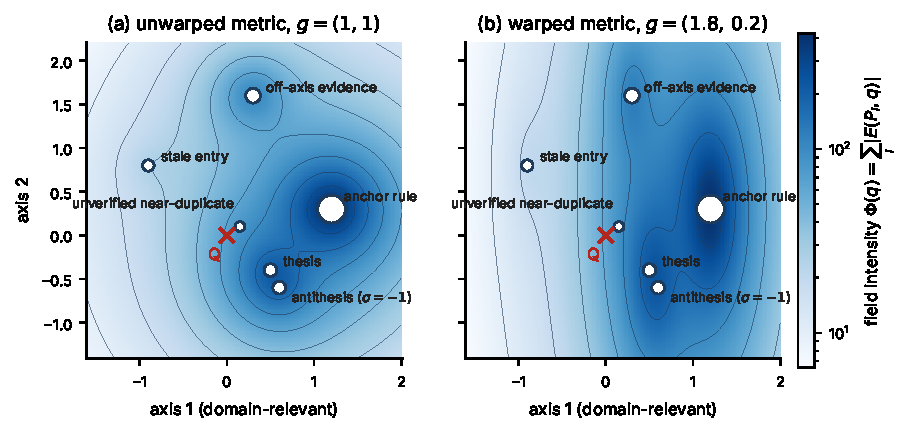
\includegraphics[width=\textwidth]{figures/field}
  \caption{Field intensity $\Phi(q)=\sum_i|\act(P_i,q)|$ over the plane of the toy memory (log colour scale; marker area grows with mass; the query $Q$ sits at the origin). (a)~Uniform metric. (b)~Query-warped metric $g=(1.8,0.2)$: axis~2 is compressed, so the field is stretched vertically and the off-axis evidence moves into reach of the query.}
  \label{fig:field}
\end{figure}

\paragraph{Reduction to cosine (Proposition~\ref{prop:cosine}).}
For $200$ random unit vectors in $d=32$ with uniform mass and $20$ random queries, the ranking by $\act$ and the ranking by cosine similarity coincide for every query (Kendall $\tau=1.00$ in all $20$ cases).

\paragraph{Mass against proximity (Proposition~\ref{prop:exchange}).}
Table~\ref{tab:exchange} places a near-duplicate ($D=0$, $m=1$) against a pattern at $D=1$ with mass $M$. The winner flips exactly at $M=(1+\epsilon)/\epsilon$: with $\epsilon=0.01$ even a $20\times$ heavier anchor loses to a duplicate; with $\epsilon=1$ a $5\times$ heavier one wins.

\begin{table}[htbp]
  \centering
  \caption{Mass--proximity exchange: which pattern activates more strongly, a near-duplicate of the query with mass $1$ or a pattern at distance $D=1$ with mass $M$, as a function of $\epsilon$.}
  \label{tab:exchange}
  \begin{tabular}{@{}rrrl@{}}
\toprule
$\epsilon$ & $(D+\epsilon)/\epsilon$ & $M$ & winner \\
\midrule
0.01 & 101 & 5 & duplicate \\
0.01 & 101 & 20 & duplicate \\
0.01 & 101 & 200 & anchor \\
0.1 & 11 & 5 & duplicate \\
0.1 & 11 & 20 & anchor \\
0.1 & 11 & 200 & anchor \\
1 & 2 & 5 & anchor \\
1 & 2 & 20 & anchor \\
1 & 2 & 200 & anchor \\
\bottomrule
\end{tabular}

\end{table}

\paragraph{Contradiction valence (Section~\ref{sec:valence}).}
Table~\ref{tab:valence} lists the activations in the scene. The antithesis has the third-largest magnitude and enters the active set at rank~3 with sign $-1$; ranking by signed $\act$ would put it last, below the stale entry at $\act=0.43$. The anchor rule, $1.24$ units away ($D=1.530$), outranks the near-duplicate $0.18$ units away ($D=0.0325$) because its mass-to-distance ratio $40/(1.530+0.1)=24.54$ exceeds the duplicate's $1/(0.0325+0.1)=7.55$: the trade-off of \eqref{eq:exchange}, with the duplicate's small but non-zero distance included.

\begin{table}[htbp]
  \centering
  \caption{Activations in the toy scene for the query at the origin, ordered by $|\act|$. The sign is the valence label handed to the rule core.}
  \label{tab:valence}
  \begin{tabular}{@{}llr@{}}
\toprule
Pattern & valence $\sigma$ & $E(P_i,Q)$ \\
\midrule
anchor rule & $+1$ & $24.54$ \\
thesis & $+1$ & $19.61$ \\
antithesis & $-1$ & $-12.20$ \\
unverified near-duplicate & $+1$ & $7.55$ \\
off-axis evidence & $+1$ & $2.91$ \\
stale entry & $+1$ & $0.43$ \\
\bottomrule
\end{tabular}

\end{table}

\paragraph{Decay and reinforcement (Section~\ref{sec:decay}).}
Table~\ref{tab:decay} follows three patterns at the query position over $60$ time units (days). The unreinforced unit-mass pattern keeps $55\%$ of its activation, the one reinforced at $t=30$ keeps $74\%$, and the $m=50$ anchor keeps $98\%$ with no reinforcement at all.

\begin{table}[htbp]
  \centering
  \caption{Decay over $60$ time units (days) with $\lambda_0=0.02\text{ days}^{-1}$, $m_\ast=1$.}
  \label{tab:decay}
  \begin{tabular}{@{}lrr@{}}
\toprule
Pattern & $\lambda_i$ & $E(t{=}60)/E(t{=}0)$ \\
\midrule
m=1, never reinforced & $0.0100$ & $0.549$ \\
m=1, reinforced at t=30 & $0.0100$ & $0.741$ \\
m=50 anchor, never reinforced & $0.0004$ & $0.977$ \\
\bottomrule
\end{tabular}

\end{table}

\paragraph{Warped metric (Remark~\ref{rem:concentration}).}
Table~\ref{tab:warp} compares the uniform metric with $g=(1.8,0.2)$. Compressing axis~2 brings the off-axis evidence from $D=2.65$ to $D=0.67$ and moves it from rank~5 to rank~4, past the near-duplicate; the anchor rule, which lies along the stretched axis, drops to rank~2 behind the thesis.

\begin{table}[htbp]
  \centering
  \caption{Warped distances and active-set ranks (by $|\act|$) for the toy scene under the uniform and the warped metric.}
  \label{tab:warp}
  \begin{tabular}{@{}lrrrr@{}}
\toprule
Pattern & $D_{g=(1,1)}$ & rank & $D_{g=(1.8,0.2)}$ & rank \\
\midrule
anchor rule & 1.530 & 1 & 2.610 & 2 \\
unverified near-duplicate & 0.033 & 4 & 0.043 & 5 \\
thesis & 0.410 & 2 & 0.482 & 1 \\
antithesis & 0.720 & 3 & 0.720 & 3 \\
off-axis evidence & 2.650 & 5 & 0.674 & 4 \\
stale entry & 1.450 & 6 & 1.586 & 6 \\
\bottomrule
\end{tabular}

\end{table}

\paragraph{Distance concentration.}
Table~\ref{tab:concentration} measures, for $2000$ random unit vectors and one random query, the spread of $D$ and the range of the distance term $-\log(D+\epsilon)$ as the dimension grows. At $d=2048$ over $2000$ samples, the distance term spans $0.15$ nats, against $\log(1+\beta)=0.69$ nats for valence ($\beta=1$) and $\log 100 = 4.6$ nats for a mass scale from $1$ to $100$: in this random-vector sample the range of the distance term is a small fraction of the mass and valence ranges; which term decides a given pair depends on their actual values. Real embeddings are not isotropic; how strongly they concentrate must be measured on the embeddings in use, but the direction of the effect is expected to be the same.

\begin{table}[htbp]
  \centering
  \caption{Concentration of squared distances $D$ from a random unit query to $2000$ random unit vectors, and the resulting dynamic range of the distance term in \eqref{eq:loglinear} ($\epsilon=0.1$).}
  \label{tab:concentration}
  \begin{tabular}{@{}rrrrr@{}}
\toprule
$d$ & $\min D$ & $\max D$ & $(\max D-\min D)/\bar{D}$ & range of $-\log(D+\epsilon)$ (nats) \\
\midrule
2 & 0.000 & 4.000 & 1.97 & 3.71 \\
8 & 0.255 & 3.883 & 1.78 & 2.42 \\
32 & 0.953 & 3.274 & 1.15 & 1.16 \\
128 & 1.431 & 2.597 & 0.58 & 0.57 \\
512 & 1.695 & 2.313 & 0.31 & 0.30 \\
2048 & 1.854 & 2.160 & 0.15 & 0.15 \\
\bottomrule
\end{tabular}

\end{table}

\section{Execution}
\label{sec:execution}

Evaluating \eqref{eq:field} over $n$ patterns costs $O(nd)$ with no data dependence between patterns: the computation is independent per pattern and runs on portable code (vectorised NumPy on CPU, or a straightforward per-pattern GPU kernel), with dedicated hardware engines for continuous field evaluation proposed only as a future design. For auditing we run the reference implementation in an isolated environment with fixed seeds and resource limits so that floating-point outputs are reproducible; wall-clock timings still depend on the underlying host hardware.

\section{Limitations and Falsification}
\label{sec:limits}

\paragraph{No empirical benchmark evaluation.}
Nothing in this paper demonstrates empirically that the RCF retrieves better on standard benchmarks than cosine similarity, than the additive score of generative agents \citep{park2023generative}, or than BM25 \citep{robertson2009bm25}, nor does this paper present physical measurements of the physical claim in Section~\ref{sec:physical_claim}. The worked example demonstrates the mathematical mechanisms of the static model on six points.

\paragraph{Undefined learned components.}
$g(Q)$, $\sigma_i(Q)$ and $\kappa_i(Q)$ are inputs to the model, not outputs of it. The model's usefulness is bounded by theirs, and NevIR \citep{weller2024nevir} shows that the contradiction signal in particular is hard to obtain from embeddings alone.

\paragraph{Distance concentration.}
Remark~\ref{rem:concentration} and Table~\ref{tab:concentration} show that the inverse-distance term loses its range in high dimension. Whether query warping restores useful discrimination (and not merely numerical spread) on real embeddings is an open empirical question.

\paragraph{Calibration of mass and numerical range.}
Masses are on an arbitrary scale, and by Proposition~\ref{prop:exchange} their scale relative to $\epsilon$ determines behaviour. A validation protocol that produces masses on a defined scale (for instance, $m_0=0.01$ at ingestion and $+1$ per independent human confirmation) is required before deployment. Moreover, Lemma~\ref{lem:bound} holds in exact arithmetic only: in IEEE-754 double precision, extreme combinations of inputs (for example a large mass at zero distance with a tiny $\epsilon$) can overflow, and a large $\lambda_i\Delta t_i$ underflows to zero. The reference implementation checks the domains (A1)--(A4) and rejects non-finite values in every numeric input and update, but does not bound their magnitudes; log-domain scoring and the archival policy of Section~\ref{sec:decay} are implementation options, not features of this release.

\paragraph{Hypothesis on extension to physical systems.}
As part of our central hypothesis (Section~\ref{sec:physical_claim}), we propose that the RCF primitives map onto physical information systems where carriers possess effective energy density ($m_i$), undergo thermodynamic relaxation and entropic decay ($\lambda_i$), and interact under structural constraints ($g(Q)$). In the present work this extension is a theoretical hypothesis, not a demonstrated physical result; testing it requires a discriminating physical test meeting the requirements stated in Section~\ref{sec:physical_tests}, and the interactive $N$-body formulation in Appendix~\ref{sec:dynamic_field}.

\paragraph{Not yet gravity in the static model.}
A gravitational system has three features the static RCF of Section~\ref{sec:model} lacks: bodies attract \emph{each other}, their positions \emph{evolve}, and mass curves the space \emph{for everyone}. In the static model only the query acts, nothing moves, and only the query rescales the metric; the activations of different patterns are computed independently, so the static field is not an $N$-body problem and should not be described as one. Turning it into an interactive dynamic field---where pattern--pattern pull governs mass shares, positions drift and relax with hysteresis, and a short-range repulsion discourages coalescence---is formulated as a theoretical design in Appendix~\ref{sec:dynamic_field}.

\paragraph{What would falsify the computational hypothesis.}
Separately from the requirements for a discriminating physical test in Section~\ref{sec:physical_tests}, the static computational model is falsifiable by five retrieval experiments: (i)~On a retrieval benchmark such as BEIR \citep{thakur2021beir}, the RCF with equal positive mass, $g\equiv 1$, and the NLI stage and decay switched off must produce rankings identical to the cosine baseline up to ties (Proposition~\ref{prop:cosine}); any deviation is a bug. (ii)~With $g(Q)$ parameterised as $g(Q)=d\cdot\operatorname{softmax}(Wq)$ and trained by pairwise ranking loss on training relevance judgments, held-out nDCG@10 must exceed the cosine baseline on the same embeddings at stated parameter and latency cost; if it does not, query warping is not worth its cost. (iii)~On NevIR \citep{weller2024nevir} (where each instance is a two-document pair, so recall at $k\ge 2$ is trivially~$1$) we evaluate pairwise sign accuracy using $\sigma,\kappa$ from an NLI model, and on a multi-document counter-argument corpus \citep{wachsmuth2018retrieval} we compare recall of contradicting passages in $A_k(Q)$ under magnitude ranking ($|\act|$) against signed-$\act$ ranking and cosine retrieval supplied with the \emph{same} NLI signal; if magnitude ranking does not beat those baselines, the magnitude policy adds nothing beyond the NLI detector. (iv)~On a corpus with time stamps (in days) and human validation labels, the multiplicative decay must beat the additive recency of generative agents at equal parameter count; if it does not, the multiplicative coupling is not justified. (v)~Ablating each term of \eqref{eq:loglinear} must cost measurable quality; a term whose removal costs nothing should be removed from the model.

\section{Conclusion}

This paper has presented the author's central hypothesis---that intelligence is an active force in the universe, that information is a substance with an equivalence to energy, and that cognitive structures exert gravity and perform structural work in an $N$-dimensional space that affects outcomes in the material world---and has translated that framework into the computable Relativistic Cognitive Field (RCF). In the demonstrated static scoring model, validated mass, signed valence, a query-warped metric and reinforcement-reset decay combine multiplicatively into a single bounded activation. Its logarithm is a linear combination of four classical retrieval signals; with the extra terms switched off (equal positive mass, $g\equiv 1$, equal valence, equal $\Delta t$, unit norm) it produces the same ranking as cosine retrieval; its smoothing constant is the exchange rate between validation and proximity; and it retrieves contradictions by magnitude and labels them by a three-valued sign rather than suppressing or averaging them away. We have stated the physical claim, proposed tests of its computational consequences and the requirements for a discriminating physical test, proved the elementary properties of the static computational model, reproduced every number and figure of the worked example in a portable reference implementation, and formulated the continuous dynamic extension as a theoretical design in Appendix~\ref{sec:dynamic_field}.

\paragraph{Acknowledgements.}
The author acknowledges the use of AI assistants (Anthropic Claude, Google Gemini, and OpenAI GPT) for drafting support, code iteration, and read-only verification checks during the preparation of this manuscript.

\section*{Reproducibility}

The reference implementation, its test suite, and the script that generates every table and figure in Section~\ref{sec:example} are included as ancillary files with this submission (\texttt{anc/}) and are published, with the paper sources, at \url{https://github.com/balgurov/relativistic-cognitive-field} (release v1.0).

\bibliographystyle{plainnat}
\bibliography{references}

\appendix
\section{Reference Implementation}
\label{app:code}

Abridged core of the reference implementation (NumPy, file \texttt{anc/rcf/field.py}). The full version validates every input against assumptions (A1)--(A4): masses below the ingestion floor $m_0 > 0$ (default $m_0=0.01$), negative metric weights, valence values outside their domains, non-positive $\epsilon$, non-finite values in any numeric input or update, assessed signs outside $\{-1,+1\}$, future-dated $t_i$ (at ingestion when the current time is given, and at retrieval), negative mass increments and non-positive validation increments all raise \texttt{ValueError}. It provides \texttt{preselect\_candidates} for the exact decayed bound~\eqref{eq:candidates}, \texttt{touch(idx, now)} for a clock reset on use, and \texttt{validate(idx, now, mass\_delta)} for a human validation event; the library records the event it is told about and does not itself authenticate a human. The label of an active-set member is taken from the supplied assessment, never inferred from the sign of $\act$.

\begin{lstlisting}[language=Python]
def warped_distance(q, coords, g=None):
    diff = coords - q
    if g is None:
        return np.sum(diff * diff, axis=-1)
    if np.any(g < 0):
        raise ValueError("metric weights must be non-negative")
    return np.sum(g * diff * diff, axis=-1)

def valence(sigma, kappa, beta):
    return sigma * (1.0 + beta * kappa)

def activation(field, q, now, g=None, sigma=None, kappa=None):
    sigma = np.ones(field.n) if sigma is None else sigma
    kappa = np.zeros(field.n) if kappa is None else kappa
    gamma = valence(sigma, kappa, field.beta)
    d2 = warped_distance(q, field.coords, g)
    dt = now - field.last_reinforced
    rate = field.lambda0 / (1.0 + field.mass / field.mass_ref)
    return field.mass * gamma / (d2 + field.eps) * np.exp(-rate * dt)

def preselect_candidates(field, q, now, k, g=None):
    s = np.abs(activation(field, q, now, g))
    kth = np.sort(s)[::-1][min(k, s.size) - 1]
    return np.flatnonzero(s >= kth / (1.0 + field.beta))

def active_set(E, k, sigma=None, assessed=None):
    order = np.argsort(-np.abs(E), kind="stable")[:k]
    if sigma is None or assessed is None:
        return order, ["unassessed"] * len(order)
    return order, [int(sigma[i]) if assessed[i] else "unassessed" for i in order]
\end{lstlisting}

\section{Design Appendix: The Dynamic Cognitive Field}
\label{sec:dynamic_field}

\emph{Design note: The continuous dynamic field outlined below is a theoretical design formulation. It is not yet implemented or tested in the accompanying reference code package; all statements below are design specifications and one worked example for the next stage of work.}

\subsection{Conceptual Model}
In the dynamic design, the memory base is treated as an interacting system in $\R^d$ with time measured in days. Each pattern $P_i$ has a current position $p_i(t)$, a rest position $r_i(t)$, a last-touch timestamp $t_i$, and a positive mass share $m_i > 0$. Total mass is conserved ($\sum_{i=1}^n m_i = M_{\text{tot}} = n$), so mass is redistributed among patterns rather than created unboundedly. A query or a human teaching enters as a visiting body $B$ at coordinates $q$ with mass $m_B$: it pulls patterns, shifts coordinates, and leaves a permanent trace in the rest positions (hysteresis) before the field relaxes back toward rest between visits.

\subsection{Mathematical Formulation of the Candidate Dynamic Design}

\paragraph{1.\ Pull kernel and self-consistent mass (with human trust prior).}
Let $D_{ij} = \|p_i - p_j\|_2^2$ and define the softened pull kernel $W_{ij} = 1/(D_{ij} + \epsilon)$ for $i\neq j$, with $W_{ii}=0$. Pure mutual pull ($m = c\,W m$) is positive and unique by the Perron--Frobenius theorem, but it lets a dense cluster of unverified near-duplicates take most of the total mass by repetition alone. To anchor mass in human validation while allowing cluster consolidation, let $\hat{\mu}\in\R^n_{>0}$ ($\sum_i \hat{\mu}_i = 1$) be the human trust prior (incremented by human confirmations) and let $\tilde{W}_{ij} = W_{ij}/\sum_k W_{kj}$ be the column-normalised pull matrix. For a coupling share $\alpha\in[0,1)$, the mass vector satisfies
\begin{equation}
\label{eq:dyn_mass}
m \;=\; (1-\alpha)\,M_{\text{tot}}\,\hat{\mu} \;+\; \alpha\,\tilde{W}\,m, \qquad \sum_{i=1}^n m_i = M_{\text{tot}}.
\end{equation}
This system has a unique strictly positive solution with $m_i \ge (1-\alpha)M_{\text{tot}}\hat{\mu}_i$, conservatively bounding mass concentration by geometry: for $\alpha\to 1$ with minimum separation $D_{\min}$, $m_i/m_j \le (D_{\max}+\epsilon)/(D_{\min}+\epsilon)$.

\paragraph{2.\ Overdamped motion, rigidity, and short-range repulsion.}
During a visit of duration $h = 1\text{ day}$ by a visitor $B$ at $q$ with mass $m_B$, each pattern moves under overdamped dynamics with rigidity proportional to its mass $m_i$ (departing from Newton's third law on purpose, since heavy anchors should resist displacement while pulling light patterns). Pure attraction lets neighbouring patterns merge; we therefore include a short-range repulsive core at separation scale $D_0 > 0$:
\begin{equation}
\label{eq:dyn_kernel}
f(D) \;=\; \frac{1}{(D+\epsilon)^{3/2}} \;-\; \frac{D_0+\epsilon}{(D+\epsilon)^{5/2}},
\end{equation}
so that pair forces vanish at $D = D_0$ and repel for $D < D_0$. The displacement over step $h$ is
\begin{equation}
\label{eq:dyn_motion}
\delta_i \;=\; \frac{\mu\,h}{m_i}\,A_i, \qquad
A_i \;=\; \sum_{j\neq i} m_j\,f(D_{ij})\,(p_j - p_i) \;+\; m_B\,\frac{q - p_i}{(D_{iq}+\epsilon)^{3/2}},
\end{equation}
where $\mu > 0$ is the mobility. A step is taken only if $\max_i \|\delta_i\|_2 < \sqrt{S_{\text{pre}}}$, with $S_{\text{pre}}$ the mean squared spread of the positions before the step; this keeps the current positions from collapsing to one point, and before each rescaling of paragraph~4 the rest positions are also checked for a positive spread. These are runtime guards, not a stability proof. The formulation requires $n\ge 2$. The softened repulsion discourages coalescence but does not guarantee a minimum separation. Contradicting patterns ($\sigma_i = -1$) are held in place during the visit displacement in the baseline design (relaxation and rescaling may still move them), or optionally repelled as a testable variant.

\paragraph{3.\ Permanence (hysteresis) and relaxation.}
A fraction $\eta\in[0,1]$ of each visit's displacement (small for queries, larger for teachings) is retained permanently in the rest position, and between visits over elapsed time $\Delta t$ (in days) positions relax exponentially toward rest at the mass-slowed rate $\lambda_i$:
\begin{equation}
\label{eq:dyn_relax}
r_i \leftarrow r_i + \eta\,\delta_i, \qquad
p_i(t+\Delta t) \;=\; r_i + (p_i(t) - r_i)\,e^{-\lambda_i\,\Delta t}, \qquad
\lambda_i = \frac{\lambda_0}{1 + m_i/m_\ast}.
\end{equation}

\paragraph{4.\ Global balance and frozen-limit readout.}
After each step, both current positions $p_i$ and rest positions $r_i$ are rescaled about their respective centroids so that the mean squared spread equals $S_0$; each rescaling requires a positive spread. Rescaling both clouds is what keeps the rest positions from drifting outward under repeated visits. At readout, activation is evaluated by the static formula~\eqref{eq:field} on the current snapshot. The static model of Section~\ref{sec:model} is recovered exactly when, in addition to $\mu=0$ and $\eta=0$ with frozen masses, the positions start at rest ($p_i=r_i$) with their mean squared spread already equal to $S_0$ (otherwise the rescaling of this paragraph must be disabled), so that relaxation and rescaling change nothing.

\paragraph{5.\ Open design choices for implementation.}
Five architectural choices remain open for empirical comparison in the next stage: (i)~entering human validation as a trust prior $\hat{\mu}$ inside the eigenvector equation~\eqref{eq:dyn_mass} versus adding human mass on top of a bounded pull share; (ii)~combining global spread rescaling with the repulsive core~\eqref{eq:dyn_kernel} versus either mechanism alone; (iii)~setting a smaller hysteresis fraction $\eta$ for queries than for teachings versus a uniform or teaching-only $\eta$; (iv)~holding contradicting patterns ($\sigma_i=-1$) in place during a visit versus actively repelling them; and (v)~overdamped memoryless motion~\eqref{eq:dyn_motion} versus carrying momentum between visits.

\subsection{A Six-Item Example of the Mass Equation}
The mass equation~\eqref{eq:dyn_mass} and the static readout~\eqref{eq:field}, evaluated on a six-pattern scene in $d=4$ with axes $(\text{Home}, \text{Sea}, \text{Sky}, \text{Tradition})$, $\epsilon=0.5$, $\alpha=0.5$, $\beta=1$, $M_{\text{tot}}=6$, a uniform trust prior, $\Delta t_i=0$, and the query $q=(1.00,\,0.20,\,0.00,\,0.50)$ with $g\equiv 1$ (Table~\ref{tab:dynscene}), give:
\begin{table}[htbp]
  \centering
  \caption{Inputs of the six-item example: coordinates and the assessment of each item for the house query (unassessed items use $\gamma=+1$).}
  \label{tab:dynscene}
  \begin{tabular}{@{}lrrrrll@{}}
  \toprule
  Item & Home & Sea & Sky & Tradition & $\sigma$ & $\kappa$ \\
  \midrule
  House in Kotor & 1.00 & 0.40 & 0.00 & 0.40 & $+1$ & 0.8 \\
  Sailing & 0.10 & 1.00 & 0.20 & 0.10 & unassessed & 0 \\
  Telescope & 0.00 & 0.20 & 1.00 & 0.00 & unassessed & 0 \\
  Feng shui & 0.70 & 0.00 & 0.10 & 0.90 & $+1$ & 0.8 \\
  Chi & 0.50 & 0.10 & 0.20 & 1.00 & $+1$ & 0.5 \\
  Bed by the door & 0.90 & 0.00 & 0.00 & 0.70 & $-1$ & 0.9 \\
  \bottomrule
  \end{tabular}
\end{table}
\begin{itemize}
  \item \textbf{Initial fixed-point masses:} Solving~\eqref{eq:dyn_mass} prior to teaching gives \emph{House in Kotor} $m=1.02$, \emph{Sailing} $0.81$, \emph{Telescope} $0.77$, \emph{Feng shui} $1.16$, \emph{Chi} $1.09$, and \emph{Bed by the door} $1.14$ (the Home/Tradition cluster carries higher mutual pull; the isolated Sky item is lightest).
  \item \textbf{Initial query (about the house):} Evaluating~\eqref{eq:field} ranks the contradiction \emph{Bed by the door} ($\ell = -1$) highest by magnitude at $|\act|=3.66$, followed by \emph{House} ($3.34$), \emph{Feng shui} ($2.62$), \emph{Chi} ($1.56$), \emph{Sailing} ($0.38$), and \emph{Telescope} ($0.28$).
\end{itemize}

\end{document}
